\documentclass[11pt]{beamer}

\usepackage[utf8]{inputenc} 
\usepackage[T1]{fontenc}
\usepackage{lmodern}
\usepackage{graphicx}
\usepackage[french]{babel}
\usepackage{listings}

\setbeamertemplate{blocks}[rounded][shadow=true]
\expandafter\def\expandafter\insertshorttitle\expandafter{%
    \insertshorttitle\hfill\insertframenumber\,/\,\inserttotalframenumber}

% \onehalfspacing

% Espacement des lignes
%\linespread{1.2}

% Theme
\usepackage{animate}
\usetheme{Warsaw}                                % un theme voir .../beamer/theme/
\usecolortheme{orchid}
\usecolortheme{whale}


% Numéro diapo en bas
%\setbeamertemplate{footline}[frame number]

\title[Equipe segment SOL : Chef de PROJET]{Projet DRONE}
\subtitle{Gestion de L'OS Embarqué}
\institute{ Ecole Supérieure des Technologies Electronique Informatique Infographie  }
\author{Pierre-jean \textsc{TEXIER}}
\date{13 Février 2014}
 

\hypersetup{% Modifiez la valeur des champs suivants
	pdfauthor   = {Texier Pierre-jean},%
	pdftitle    = {Présentation PROJET 2013-2014},%
	pdfsubject  = {Gestion de l'OS Embarqué et gestion de l'environnement Graphique},%
	pdfkeywords = {Mots clés},%
	pdfcreator  = {PDFLaTeX},%
	pdfproducer = {PDFLaTeX},%
}


\begin{document}
	% Diapositive
	\begin{frame}
	  \maketitle
		\begin{figure}
			\begin{center}
				\includegraphics[width=2cm]{common/estei.png}\\
				\includegraphics[width=1cm]{common/cc.png}
			\end{center}
		\end{figure}
	\end{frame}
		
	\begin{frame}
		\frametitle{Sommaire}
		%\framesubtitle{}
		\begin{columns}[t]
		\begin{column}{5cm}
		\tableofcontents[sections={1-5},hideallsubsections]
		\end{column}
		\begin{column}{5cm}
		\tableofcontents[sections={6-10},hideallsubsections]
		\end{column}
		\end{columns}
	 \end{frame}
	
	%%%%%%%%%%%%%%%%%%%%%%%%%%%%%%%
	
 	\section{Présentation du Projet}
	\begin{frame}{Présentation du Projet}
	
	\begin{itemize}
	 \item Projet de FIN d'étude
	 \pause
	 \item Mise en situation industrielle
	 \pause
	 \item 2 Composants --> 2 Equipes  
	 \pause
	 \begin{center}
		    \includegraphics[width=5cm]{common/projet.png}
	 \end{center}
	\end{itemize}
	\end{frame}
	
	%%%%%%%%%%%%%%%%%%%%%%%%%%%%%%%
	
	\section{Présentation Segment SOL}
	\begin{frame}{Présentation du Segment SOL}
		\begin{itemize}
		    \item Présentation
		    \pause
			\item L'équipe (OBS : Organization Breakdown Structure)\\
		    \pause
		    \begin{center}
			\includegraphics[width=8cm]{common/OBS.png}
		    \end{center}
		\end{itemize}
	\end{frame}
	
	%%%%%%%%%%%%%%%%%%%%%%%%%%%%%%%
	
	\subsection[]{Matrice de Compétence}
	\begin{frame}{Matrice de compétence Segment SOL}
		\begin{center}
			\includegraphics[width=10cm]{common/matrice.png}
		\end{center}
			\begin{block}{Remarques}
			  \begin{itemize}
			      \item Permet d'organiser au mieux les ressources
			  \end{itemize}
			\end{block}
	\end{frame}
		
	%%%%%%%%%%%%%%%%%%%%%%%%%%%%%%%%%%%%%%ù
	
	\section{Analyse Fonctionelle}
	\begin{frame}{Degré 1}
	\begin{center}
		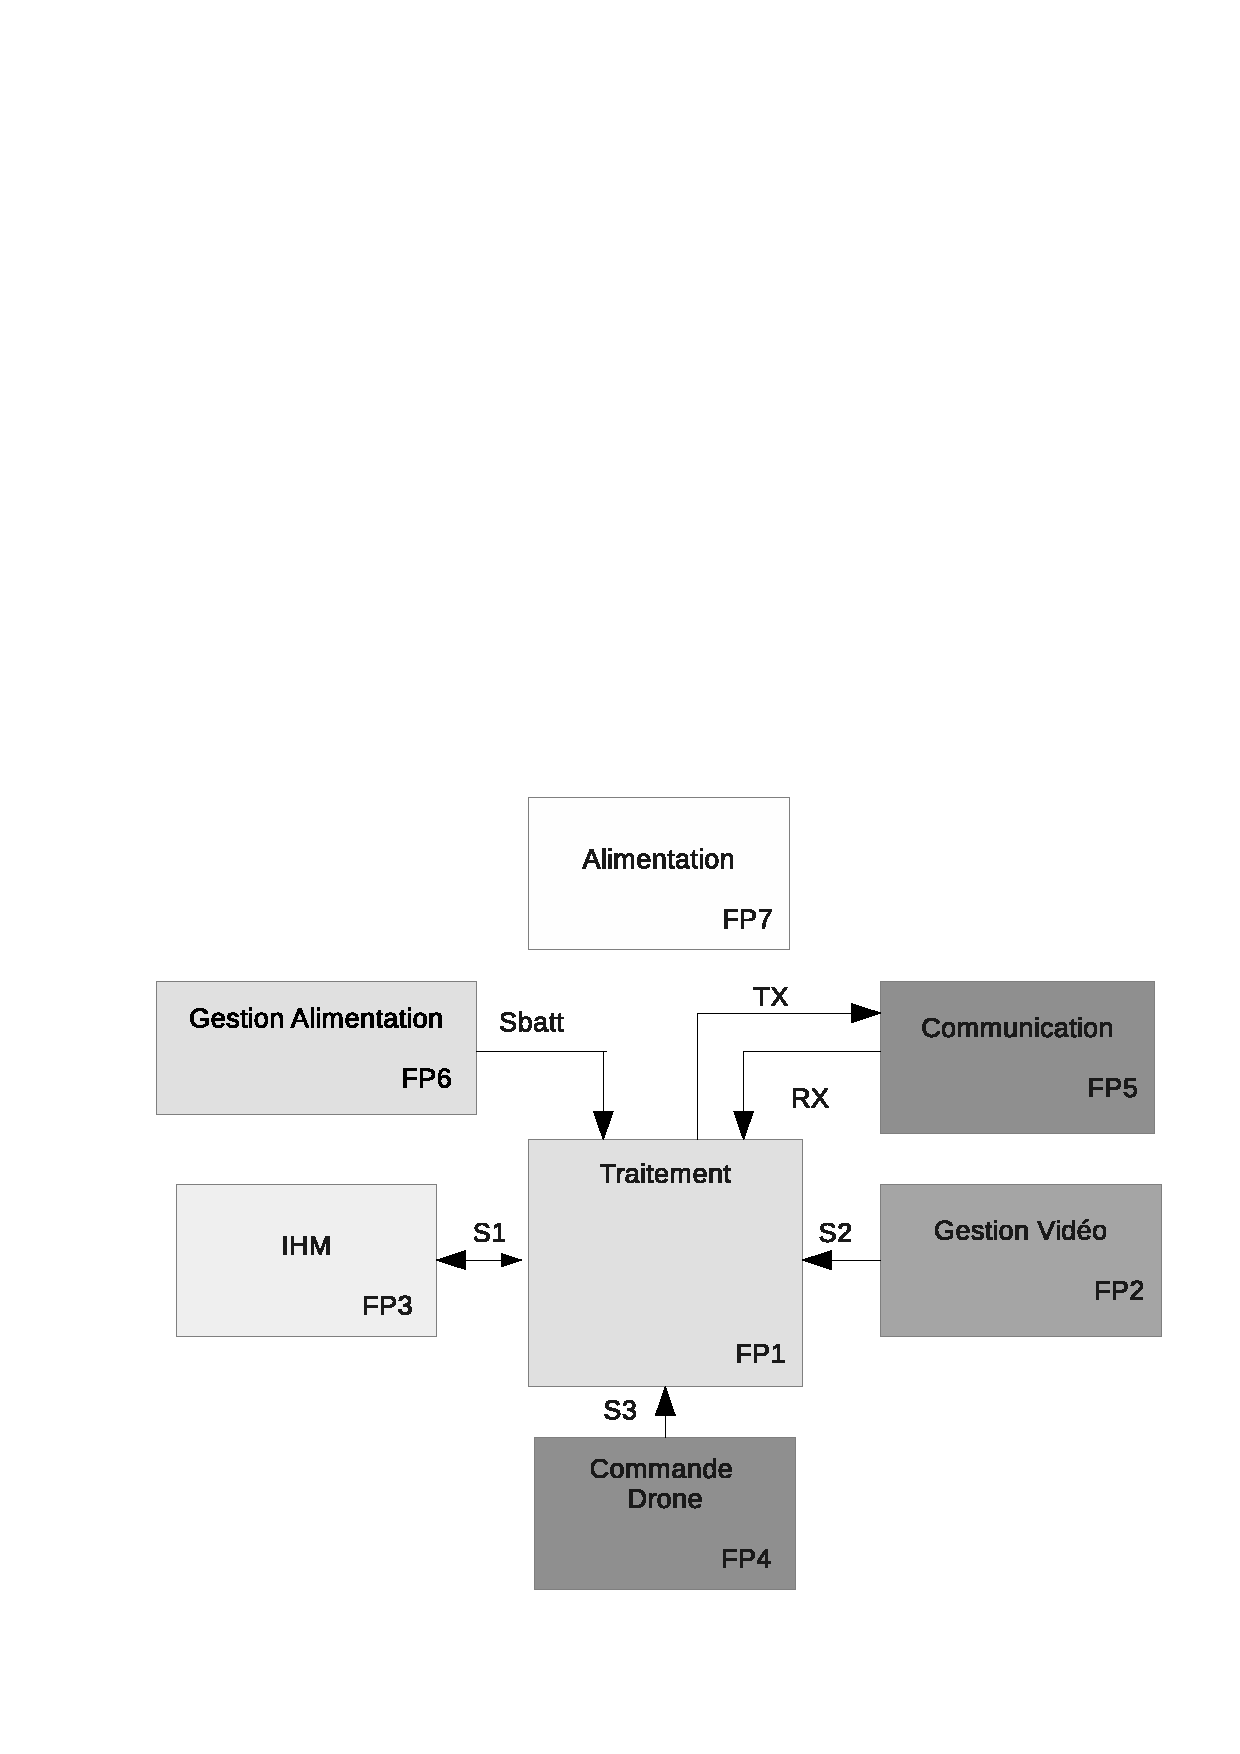
\includegraphics[width=7cm]{common/fonc.png}
	\end{center}
	\end{frame}
	
	%%%%%%%%%%%%%%%%%%%%%%%%%%%%%%%%%%%%%%ù
	
	\section{Gestion de Projet}
	\subsection{Cycle de vie Logiciel}
	\begin{frame}{Cycle de vie Logiciel}
		\begin{center}
			\includegraphics[width=10cm]{common/V.png}
		\end{center}
	\end{frame}
	
	\begin{frame}{ROADMAP : Segment SOL}
		\begin{center}
			\includegraphics[width=10cm]{common/roadmap.png}
		\end{center}
		\pause
		\begin{block}{Remarques}
		\begin{itemize}
			\item 2 Jalons : Intégration
			\item Suivi du cycle de Vie Logiciel
		\end{itemize}
		\end{block}
	\end{frame}
	
	\begin{frame}{Suivi des dépenses : Segment SOL}
		\begin{center}
			\includegraphics[width=10cm]{common/depenses.png}
		\end{center}
		\pause
		\begin{block}{Remarques}
		\begin{itemize}
			\item 750 Euros de Budget à l'instant t0
			\item Environ 450 Euros dépensé en fin de PROJET
		\end{itemize}
		\end{block}
	\end{frame}
	
	%%%%%%%%%%%%%%%%%%%%%%%%%%%%%%%
	
	\subsection{Diagramme de GANTT}
	\begin{frame}{Gantt Prévisionnel}
		\begin{center}
			\includegraphics[width=10cm]{common/Gantt.png}
		\end{center}
				
		\begin{block}{Remarques}
			\begin{itemize}
			\item Les tâches du cahier des charges sont présentées ainsi que les relations entre elles
		\end{itemize}
		\end{block}
	\end{frame}
	
	%%%%%%%%%%%%%%%%%%%%%%%%%%%%%%%
	
	\subsection{Diagramme PERT}
	\begin{frame}{Pert}
		\begin{center}
			\includegraphics[width=4cm]{common/pert.png}
		\end{center}
	\end{frame}
	
	%%%%%%%%%%%%%%%%%%%%%%%%%%%%%%%
	
	\subsection{Outils}
	\subsubsection[]{Outils mis en place}
	\begin{frame}{Outils mis en place}
	Gestion de Version
	\begin{itemize}
	 \item GIT 
	      \begin{itemize}
	      \item \href{https://github.com/estei-master/segment_SOL}{\beamergotobutton{GITHUB Segment SOL}}
	      \end{itemize}
	 \end{itemize}
	 Gestion de Documentation
	 \begin{itemize}
	 \item Doxygen 
	      \begin{itemize}
	      \item \href{http://78.231.214.8/ihm2/html/}{\beamergotobutton{Doxygen Segment SOL}}
	      \end{itemize}
	  \end{itemize}
	  Gestion de Publication 
	  \begin{itemize}
	 \item Doku-Wiki 
	    \begin{itemize}
	    \item \href{http://78.231.214.8/dokuwiki/doku.php}{\beamergotobutton{Wiki Segment SOL}}
	    \end{itemize}
	\end{itemize}
	
	\end{frame}
	
	%%%%%%%%%%%%%%%%%%%%%%%%%%%%%%%
	
	\section{Cahier des Charges}
	\begin{frame}
		\frametitle{Cahier des Charges Personnel}
		\framesubtitle{FP1 - FP6}
		\begin{center}
				\includegraphics[width=3cm]{common/cdcperso.png}	\\ 
		\end{center}
	\begin{block}{Tâches à réaliser}
		\begin{itemize}
			\item OS Linux embarqué Fonctionnel
			\item Préparation de l'environnement graphique (Qt, openCV, ...)
			\item Optimisation du temps de boot \textbf<2>{hardware} et \textbf<2>{subjectif}
			\item Gestion de l'énergie
		\end{itemize}
	\end{block}
	\end{frame}
	
	%%%%%%%%%%%%%%%%%%%%%%%%%%%%%%%
	\section{Droit}
	
	\begin{frame}{Droit}
	2 types de Licences utilisés pour le Projet
	\pause	
	\begin{itemize}
		\item GPLv3 \includegraphics[width=0.4cm]{common/gnu.png}	\\
		\href{http://www.tldrlegal.com/license/gnu-general-public-license-v3-(gpl-3)}{\beamergotobutton{Texte GPLv3}}
		
	\end{itemize}
	\pause	
	\begin{itemize}
		\item Creative Commons 	\includegraphics[width=1cm]{common/cc.png}\\
		\href{http://creativecommons.org/licenses/by-sa/4.0/}{\beamergotobutton{Texte Creative Commons}}
	\pause	
	\end{itemize}
	\begin{block}{Le plus}
			\begin{itemize}
			\item Développement avec des Outils Libre
			\item Améliore la maintenabilité, portabilité du développement
		\end{itemize}
		\end{block}
		\pause
		\begin{block}{Quelques Outils}
			\begin{itemize}
			\item GIMP, GNU Linux, GNU plot, bootchart, \LaTeX, fbvis, ...
		\end{itemize}
		\end{block}
	\end{frame}
	%%%%%%%%
	
	\section{Réalisations}
	
	\begin{frame}{Réalisations}
		
			\begin{center}
	\includegraphics[width=2cm]{common/tux.png}	
	\end{center}
		
	\end{frame}
	
	\subsection{Choix technologiques}
	\begin{frame}[label=choix]{Choix technologiques}
	\begin{itemize}
	\item \textbf<2>{S}ystem \textbf<2>{O}n \textbf<2>{C}hip\\
	\begin{center}
		  \includegraphics[width=2cm]{common/220px-AllWinner_A20.jpg}\\
		  \hyperlink{SoC}{\beamergotobutton{Synoptique}}\\
	\end{center}
	\item Carte de développement
	\end{itemize}
	\begin{center}
		  \includegraphics[width=2cm]{common/A20-OLinuXino-MICRO-0.jpg}\\
		  \hyperlink{SbC}{\beamergotobutton{Analyse des périphériques}} \hyperlink{SbC_2}{\beamergotobutton{Disponible sur le marchés}}\\
	\end{center}
	\end{frame}
	
	\subsection{Environnement}
	\begin{frame}{Environnement ``Linux Embarqué''}
	\begin{center}
	\includegraphics[width=8cm]{common/arcg.png}	
	\end{center}
	\end{frame}
	
	
	\begin{frame}{Chaine de compilation croisée}
	\begin{center}
	  \includegraphics[width=2cm]{common/linaro.jpeg}
	\end{center}
	\begin{itemize}
			\item gcc-linaro-arm-linux-gnueabihf-4.7-linux
			\includegraphics[width=1cm]{common/gnu.jpeg}
	\end{itemize}
	\begin{columns}[t]
	\begin{column}{5cm}
	\begin{block}{Pourquoi armhf ?}
		FPU neon-vfvp4
	\end{block}
	\end{column}
	\begin{column}{5cm}
	\begin{block}{Possibilitées}
	\begin{itemize}
	      \item CodeSourcery
	      \item Crosstool-ng
	      \item Buildroot
	\end{itemize}
	\end{block}
	\end{column}
	\end{columns}
	\end{frame}
	
	\begin{frame}{Risques et Opportunités}
	\begin{center}
	  \includegraphics[width=8cm]{common/risques.png}\\
	\end{center}
	\end{frame}
	

	
	\subsection{Kernel}
	\begin{frame}[label=Kernel]{Kernel}
	Kernel ? \\ \hyperlink{Linux}{\beamergotobutton{Linux}}\\
	\pause
	Pourquoi ?
	\pause
	 \begin{itemize}
	  \item Empreinte Mémoire
	  \pause
	  \item Besoins pour le Projet (V4L, Tactile, ...)
	 \end{itemize}
	  \pause
		\begin{block}{Informations}
		\begin{itemize}
			\item Version 3.4.67
			\item Non mainline \\
			\href{https://github.com/linux-sunxi/linux-sunxi}{\beamergotobutton{Lien github}}
		\end{itemize}
		\end{block}
	\end{frame}
	
	\begin{frame}{Configuration}
	 \begin{itemize}
	  \item Xconfig
	  \item 5.20 MB --> 3.33 MB
	 \end{itemize}
	\includegraphics[width=3cm]{common/tuxleg.png}\\
	\end{frame}
	
	\begin{frame}{Configuration}
	 \begin{itemize}
	  \item Xconfig
	  \item 5.20 MB --> 3.33 MB
	 \end{itemize}
	\includegraphics[width=3cm]{common/SD.png}\\
	\end{frame}
	
	%%%%%%%%%%%%%%%%%%%%%%%%%%%%%%%
	
	\subsection{Qt embedded}
	\begin{frame}[label=pageQt]{Qt embedded}
	 \includegraphics[width=1cm]{common/Qt.jpeg}\\
			  Portage sur cible Arm Cortex A7 : 
		\begin{itemize}
		\pause
			  \item<+-|alert@+> Librairie touchscreen tslib \hyperlink{tslib}{\beamergotobutton{tslib}}\\
			  \item<+-|alert@+> Qt embedded 4.8.2 \hyperlink{Qt}{\beamergotobutton{Qt}}\\
			  
		\end{itemize}
	\end{frame}
	

	
	%%%%%%%%%%%%%%%%%%%%%%%%%%%%%%%
	
	\subsection{OpenCV embedded}
	\begin{frame}[label=pageopenCV]{OpenCV embedded}
	\includegraphics[width=1cm]{common/opencv.png}\\
	\hyperlink{openCV}{\beamergotobutton{openCV}}\\
		\begin{center}
			
		\end{center}
	\end{frame}
	
	
	%%%%%%%%%%%%%%%%%%%%%%%%%%%%%%%
	
	\subsection{Optimisation démarrage}
	\subsubsection[]{Hardware}
	\begin{frame}[label=optimisation]{Hardware}
	U-boot
	\begin{itemize}
			\item Variable 'bootdelay'
	\end{itemize}
	Scripts de démarrage : \hyperlink{bootchart}{\beamergotobutton{bootchart}}\\
	\begin{itemize}
			\item Networking
			\item ssh
			\item exim4
			\item apache
	\end{itemize}
	\end{frame}
	\subsubsection[]{Subjectif}
	\begin{frame}{Subjectif}
	Remplacement du Logo 
	\begin{itemize}
	\item Logo de base 
		\begin{center}
		 \includegraphics[width=1cm]{common/logo_1.png}
		\end{center}
	\item Logo personnalisé
		\begin{center}
		 \includegraphics[width=2cm]{common/logo_2.png}
		\end{center}
	\end{itemize}
	\end{frame}
	
	\begin{frame}{Suite ... Subjectif}
	Utilisation simpliste du Framebuffer
	\end{frame}
	%%%%%%%%%%%%%%%%%
	\subsection{Power Management}
	\begin{frame}[fragile]{Power Management}
	\begin{itemize}
			\item Composant --> AXP209\\
			\item Création d'un `Cron'
				\begin{block}{}
				*/2 * * * * /bin/bash /home/PJ/power-management.sh\\
				\end{block}
	\end{itemize}
	\begin{center}
		\includegraphics[width=4cm]{common/power_management.png}
	\end{center}
	\end{frame}
	%%%%%%%%%%%%%%%%%%%
	\subsection{Optimisation du Système}
	\begin{frame}{Réalisé}
	 \begin{itemize}
	 \item  Système de fichier Temporaire \\
	    	 \begin{itemize}
		    \item  \textit{tmpFS}
		  \end{itemize}
	\item Autologin \\
	  	  \begin{itemize}
		    \item  \textit{agetty --autologin}
		  \end{itemize}
	\item Lancement Automatique de l'application : ihm\\
	\item UDEV \\
	  \begin{itemize}
		    \item iDVendor
		    \item iDProduct
	  \end{itemize}
	\end{itemize}
	\end{frame}
	
	\begin{frame}{Possible}
	\begin{itemize}
	 \item Accélération matérielle 
	\begin{center}
		\includegraphics[width=2cm]{common/opengles.png}
	\end{center}
	 \item Gestion des Heuristiques
	 \pause
	 \begin{itemize}
	 \item powersave
	 \pause
	 \item fantasy
	 \pause
	 \item ondemand
	 \pause
	 \item interactive
	 \pause
	 \item userspace
	 \pause
	 \item perfomance
	 \end{itemize}
	\end{itemize}
	\end{frame}

		%%%%%%%%%%%%%%%%%%%%%%%%%%%%%%%%%%%%%%ù
	\section{Bilan de LOT}
	\begin{frame}{Bilan de LOT}
	Coût de Developpement\\
	\begin{center}
	\begin{tabular}{|c|c|}
			\hline
			Nom / Prénom & Coût\\
			\hline
			TEXIER Pierre-jean  & 3300 Euros\\
			\hline
			PRADEAU Martin  & 2719 Euros \\
			%\hline
			POUCH Pierre  & 2640 Euros \\
			%\hline
			L'HUILLIER Guillaume  & 2640 Euros \\
			%\hline
			OUKRAT Rémi  & 19 669 Euros\\
				
			\hline
			\end{tabular}
			\end{center}
	Coût D'industrialisation pour 100 Pièces --> 33905 euros

	\end{frame}
	

	\section{Conclusion}
	\begin{frame}{Conclusion}
	Compétences Acquises
		\begin{center}
		\begin{itemize}
			\item Apport ...
		\end{itemize}
		\end{center}
	Bilan Personnel
		\begin{center}
		\begin{itemize}
			\item Apport ...
		\end{itemize}
		\end{center}
	\end{frame}
	
	\subsection{Questions}
	\begin{frame}{FIN}
	Questions 
		\begin{center}
		  \includegraphics[width=2cm]{common/dialog-question.png}
		\end{center}
	Tests de Validation
		\begin{center}
		  \includegraphics[width=3cm]{common/appli.png}
		\end{center}
	\end{frame}
	
%%%%%%%%%%%%%%%%%%%%%%%%%%%%%%%%%%%%%%%%%%%%%%%%%%%%%%%%%%%%%%%%%%%
	\begin{frame}[label=Linux]{Système Linux}
	 \begin{center}
		\includegraphics[width=8cm]{common/kernel.png}
	 \end{center}
	\hyperlink{Kernel}{\beamerreturnbutton{retour}}
	\end{frame}
	
	\begin{frame}[label=SoC]{Synoptique du System On Chip}
	 \begin{center}
		\includegraphics[width=7cm]{common/SoC.png}
	 \end{center}
	\hyperlink{choix}{\beamerreturnbutton{retour}}
	\end{frame}
	
	\begin{frame}[label=SbC]{Analyse des périphériques}
	 \begin{center}
		\includegraphics[width=6cm]{common/Periph.png}
	 \end{center}
	\hyperlink{choix}{\beamerreturnbutton{retour}}
	\end{frame}
	
	\begin{frame}[label=SbC_2]{Etude du Marché}
	 \begin{center}
		\includegraphics[width=2.5cm]{common/rpi.jpg}
		\includegraphics[width=2.5cm]{common/Panda.png}
		\includegraphics[width=2.5cm]{common/odroid.jpg}
		\includegraphics[width=2.5cm]{common/Cubieboard.jpeg}
	 \end{center}
	\hyperlink{choix}{\beamerreturnbutton{retour}}
	\end{frame}
	
	\begin{frame}[label=Qt]{Qt embedded}
	\begin{center}
			  \includegraphics[width=8cm]{common/Qt_arch.png}
		\end{center}
		\hyperlink{pageQt}{\beamerreturnbutton{retour}}
	\end{frame}
	
	\begin{frame}[label=tslib]{tslib}
	\begin{center}
			  \includegraphics[width=6cm]{common/tslib.png}
		\end{center}
		\hyperlink{pageQt}{\beamerreturnbutton{retour}}
	\end{frame}
	
	\begin{frame}[label=openCV]{openCV}
			\begin{center}
			  \includegraphics[width=6cm]{common/v4l.png}
		\end{center}
		\hyperlink{pageopenCV}{\beamerreturnbutton{retour}}
	\end{frame}
	
	\begin{frame}[label=bootchart]{bootchart}
			\begin{center}
			  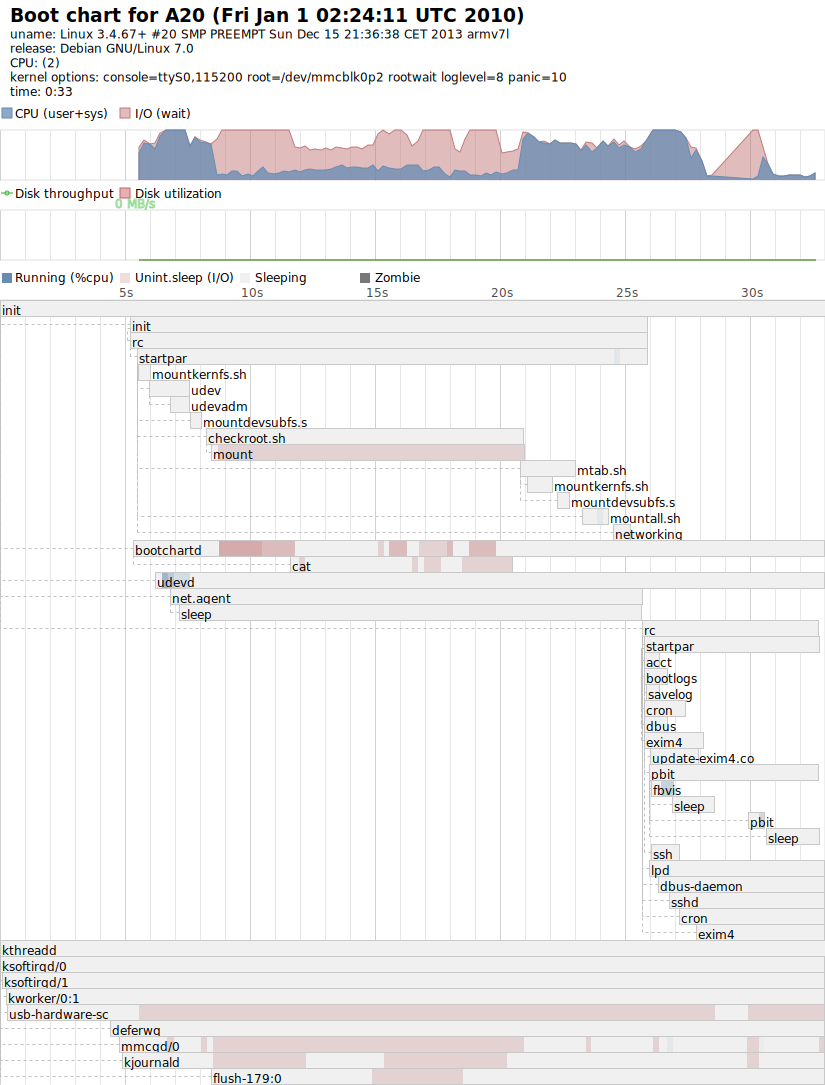
\includegraphics[width=4cm]{common/bootchart.png}
		\end{center}
		\hyperlink{optimisation}{\beamerreturnbutton{retour}}
	\end{frame}
%%%%%%%%%%%%%%%%%%%%%%%%%%%%%%%%%%%%%%%%%%%%%%%%%%%%%%%%%%%%%%%%%%%
\end{document}
